\begin{center}\section{极数}\label{chapter_number_of_poles}\end{center}
\subsection{常数项级数的概念与性质}
$\alpha$
		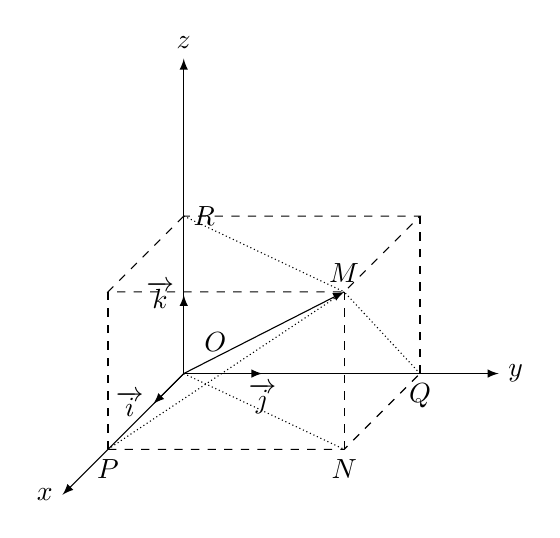
\begin{tikzpicture}[>=latex,scale=1]
	%(y,z,x)
	\node at (.4,.4,0)[]{$O$};
	\draw[->] (0,0,0)--(1,0,0)node[below]{$\overrightarrow{j}$};
	\draw[->] (0,0,0)--(0,0,1)node[left]{$\overrightarrow{i}$};
	\draw[->] (0,0,0)--(0,1,0)node[left]{$\overrightarrow{k}$};
	\draw[->] (0,0,0)--(4,0,0)node[right]{$y$};
	\draw[->] (0,0,0)--(0,0,4)node[left]{$x$};
	\draw[->] (0,0,0)--(0,4,0)node[above]{$z$};
	\draw[->] (0,0,0)--(3,2,2.5)node[above]{$M$};
	\draw[dashed] (0,0,2.5)node[below]{$P$}--(3,0,2.5)node[below]{$N$}--(3,0,0)node[below]{$Q$};
	\draw[dashed] (0,2,0)node[right]{$R$}--(0,2,2.5)--(3,2,2.5)--(3,2,0)--cycle;
	\draw[dashed](0,0,2.5)--(0,2,2.5);
	\draw[dashed](3,0,2.5)--(3,2,2.5);
	\draw[dashed](3,0,0)--(3,2,0);
	\draw[densely dotted](0,0,0)--(3,0,2.5);
	\draw[densely dotted](0,0,2.5)--(3,2,2.5);
	\draw[densely dotted](0,2,0)--(3,2,2.5);
	\draw[densely dotted](3,0,0)--(3,2,2.5);
\end{tikzpicture}